% Hamad Medical Corporation
% Georges Younes

\section{Topological Update Algorithms for Incremental Cutting of 3D Meshes}\label{sec:topological_updates}

\section{Scalable Methods for Non-linear Real-time Finite Element Simulation}\label{sec:fem_simulation}

\subsection{Discontinuous Finite Elements}\label{ssec:discontinuous_fem}
One modeling challenge in surgical simulation is the representation of cuts. There are broadly two approaches to modeling cuts. In one approach, a local region is remeshed, i.e., tetrahedral elements near the region of the cut are removed from the finite element mesh and new ones, consistent with the topology and geometry of the cuts are inserted. This is an expensive operation and might limit the real-time interaction. Another approach is to use the existing mesh, but use an extended set of basis functions in the elements where the cut is introduced. The discontinuous basis functions are simply added to the existing basis functions and this strategy has the potential for significant computational savings. We have developed a basis function for a tetrahedral element that includes a planar cut and will test the formulation and assess its effectiveness in the simulator.

\subsection{Incremental Solver}\label{ssec:incremental_solver}
At-every-iteration of the simulation, a geometric master model locates the surgical tools, resolves tool-tissue collisions and tissue-tissue collisions, and communicates this information to the finite element model. The finite element has to update the solution, including the displacements of the model and the stresses in it, based on the new geometry (cut location) and any contact constraints between tools and tissue. Resolving the finite element system from scratch with every such update would preclude real-time operation. We started the development of incremental solution strategies that exploit the nature of the changes to generate the updated displacements and stresses. These changes in the geometry and contact constraints are formulated as low rank updates of the finite element stiffness matrix.

\hrule%

\subsection{Discontinuous Finite Elements}\label{ssec:discontinuous_fem}
We developed and tested the five types of topologically-distinct discontinuous tetrahedral elements that occur during incision. The top portion of the figure below show the 1-edge, 2-edge, and 3-edge cases (involving edges sharing a vertex), while the left two pictures of bottom portion show the 3-edge and 4-edge cases (involving edges around two different vertices). These elements involve planar cuts inside individual elements. Cuts with extensive curvature along their paths are modeled accurately by refining the discretization s shown on the right of the bottom row.

\begin{figure}
  \centering%
  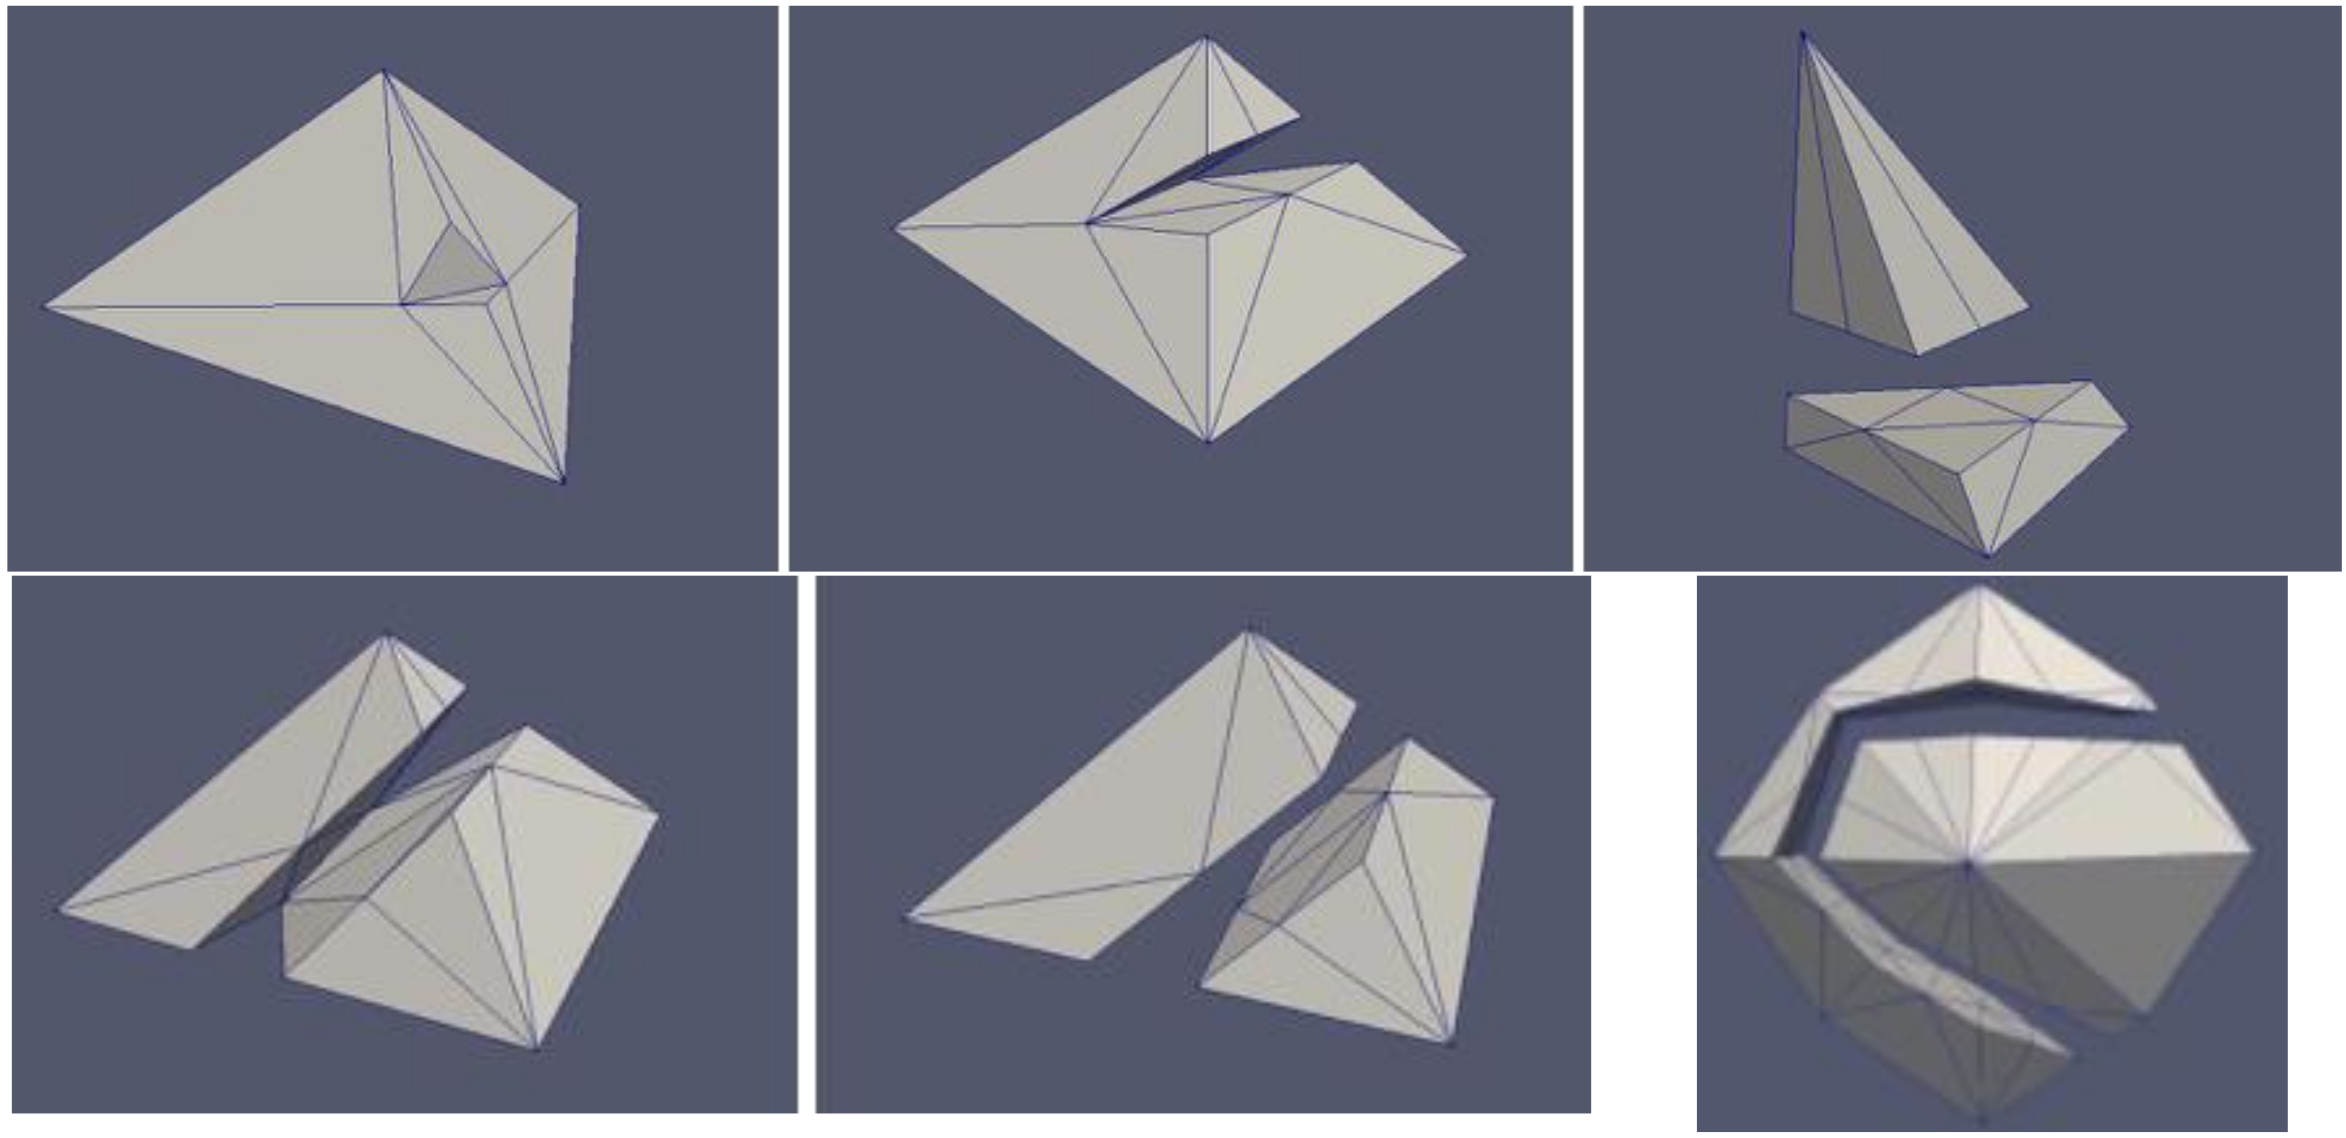
\includegraphics[width=0.85\linewidth]{simulation/cut_configurations}
  \caption{---}\label{fig:discontinuous_tetrahedra_fem}
\end{figure}

\subsection{Incremental Solver}\label{ssec:incremental_solver}
Incremental updating of the model is an important step for real-time cutting procedure simulation. The key to incremental cutting is to reuse as much state information as possible from the previous steps and express a new cut state as a minimal and low rank update of the previous one. The figure below show an example of single tetrahedral being cut incrementally,where the added sub-tetrahedra generate the necessary stiffness updates. We have finished the implementation and testing of the incremental solution strategy which relies on a state machine to change elements from one cut state to another and generate the necessary updates.

\begin{figure}
  \centering%
  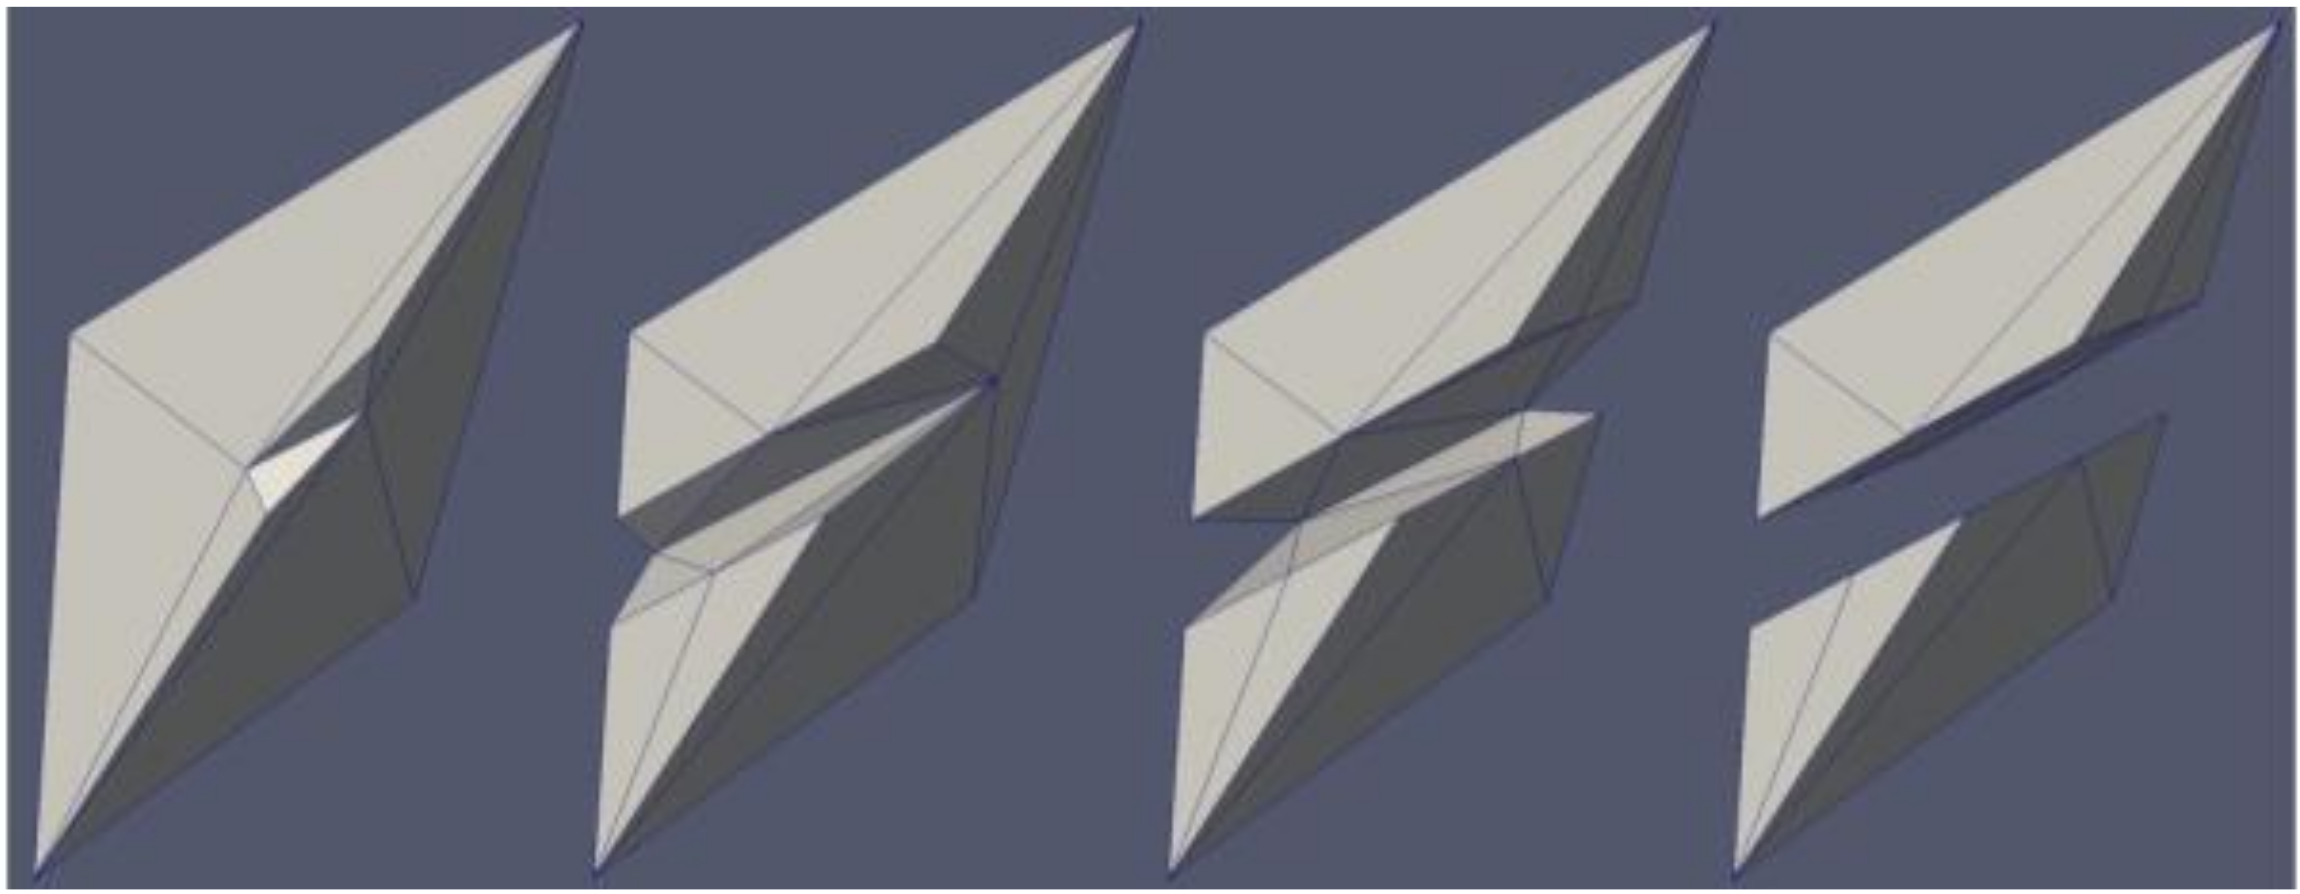
\includegraphics[width=0.7\linewidth]{simulation/cut_progression}
  \caption{---}\label{fig:discontinuous_tetrahedra_solver}
\end{figure}

\subsection{Non-linear Solver}\label{ssec:nonlinear_solver}
The nonlinear solver is necessary when large deformations take place. The solution strategy in this case involves an iterative Newton-like scheme that builds on the linear solve. The challenge for the non-linear solution is to control both the number of iterations and the cost of solving the modified linear problem at every iteration. We have started the development of a strategy that performs an approximate solution for the modified problem at every iteration, based on a hierarchical matrix representation of the stiffness matrix which produce algebraic approximations of off-diagonal matrix blocks and can substantially speed up the solution process.

\hrule%

\subsection{Non-linear Solver}\label{ssec:nonlinear_solver}
We developed and tested a solver for simulating the core nonlinear cutting procedures. The figures below illustrate the types of simulations that the solution engine supports. An idealized urethra tube is under tension and is snipped incrementally. Modifications to the underlying tetrahedral model are generated automatically as the tube is sniped around a cross section by a scissor tool (not shown). The resulting nonlinear tube deformations are shown.

\begin{figure}
  \centering%
	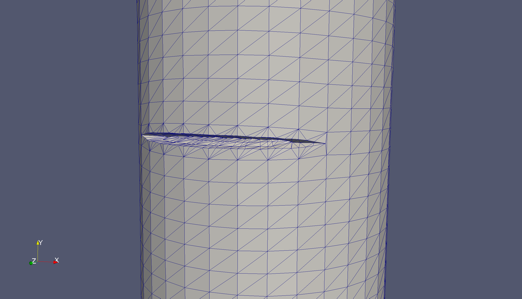
\includegraphics[width=0.49\linewidth]{simulation/tube_1}\hfill%
	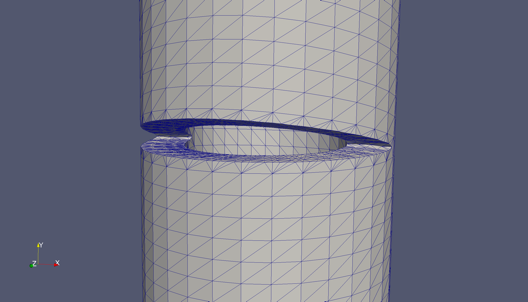
\includegraphics[width=0.49\linewidth]{simulation/tube_2}\\[1.5ex]
	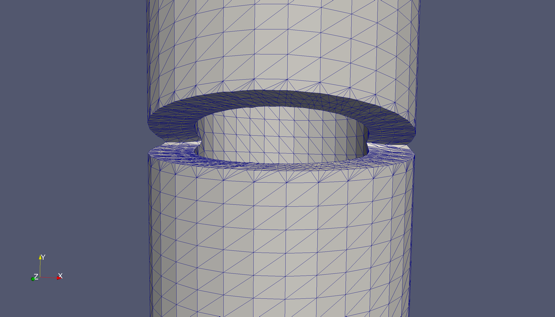
\includegraphics[width=0.49\linewidth]{simulation/tube_3}\hfill%
	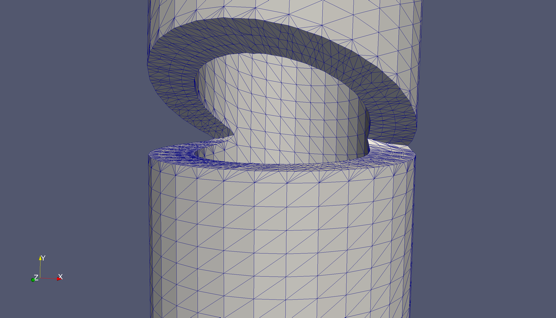
\includegraphics[width=0.49\linewidth]{simulation/tube_4}\\
	\caption{---}\label{fig:tube}
\end{figure}

We also performed a series set of stress tests to verify the robustness of the non-linear cutting and mesh modification strategies. The complex geometric nonlinearities involved in the simulation of general cut paths require a high degree of robustness in the simulator. Shown in the figure below are various cut paths of a solid sphere discretized by tetrahedral elements to demonstrate the general flexibility and reliability of our simulation engine.

\begin{figure}
  \centering%
	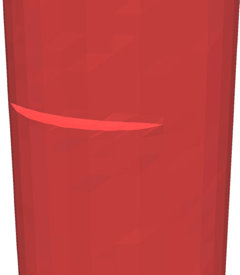
\includegraphics[width=0.22\linewidth]{simulation/tube_5}\hfill%
	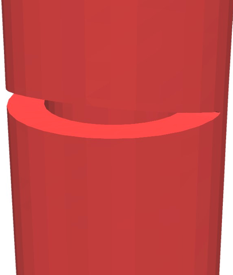
\includegraphics[width=0.22\linewidth]{simulation/tube_6}\hfill%
	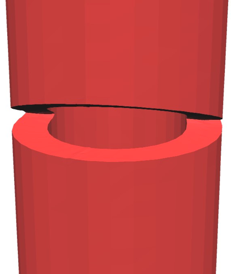
\includegraphics[width=0.22\linewidth]{simulation/tube_7}\hfill%
	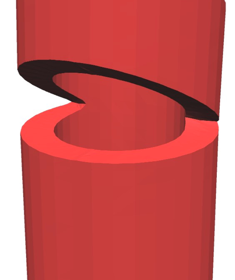
\includegraphics[width=0.22\linewidth]{simulation/tube_8}\\
	\caption{---}\label{fig:tube_stress}
\end{figure}

\begin{figure}
  \centering%
	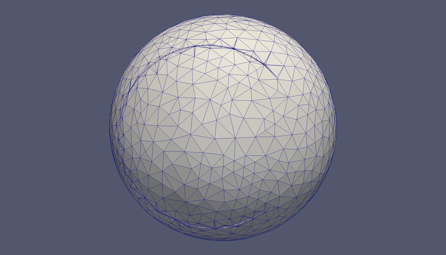
\includegraphics[width=0.49\linewidth]{simulation/sphere_1}\hfill%
	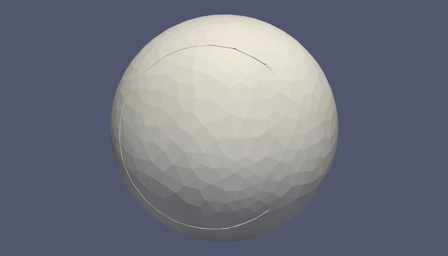
\includegraphics[width=0.49\linewidth]{simulation/sphere_2}\\[1.5ex]
	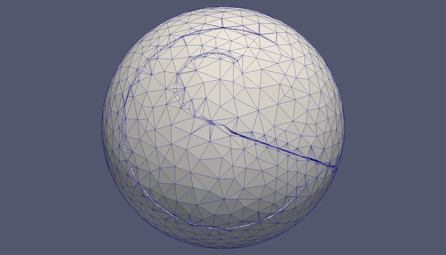
\includegraphics[width=0.49\linewidth]{simulation/sphere_3}\hfill%
	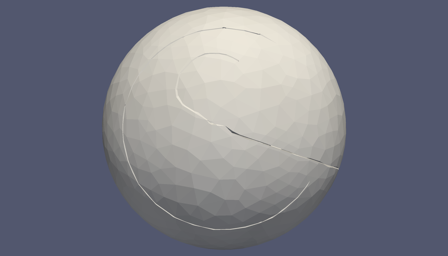
\includegraphics[width=0.49\linewidth]{simulation/sphere_4}\\[1.5ex]
	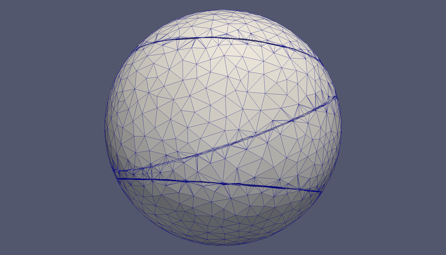
\includegraphics[width=0.49\linewidth]{simulation/sphere_5}\hfill%
	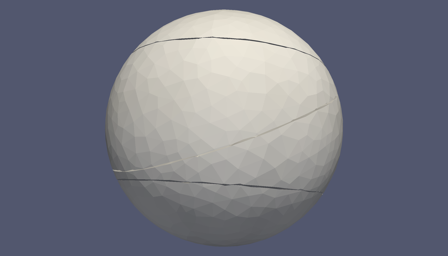
\includegraphics[width=0.49\linewidth]{simulation/sphere_6}\\
	\caption{---}\label{fig:sphere}
\end{figure}

\subsection{GPU Acceleration}\label{ssec:gpu_acceleration}

We developed and tested GPU-accelerated routines for the hierarchical matrix-vector multiplication operations involved in the finite element solution. Hierarchical matrices are space and time efficient representations of dense matrices that exploit the low rank structure of matrix blocks at different levels of granularity. The hierarchically low rank block partitioning produces representations that can be stored and operated on in near-linear complexity instead of the usual polynomial complexity of dense matrices. In the context of real-time simulation, this near-linear growth is key for the simulation of large realistic models. The figures below show how a hierarchical matrix is partitioned: some blocks (shown in red) are stored as regular dense matrices, while others of differing sizes (shown in blue/green) are stored as low rank blocks.

\begin{figure}
  \centering%
	\includegraphics[width=0.5\linewidth]{simulation/gpu_block}\vspace{2ex}
	\includegraphics[width=\linewidth]{simulation/gpu_zoom}\\
	\caption{---}\label{fig:gpu_matrix}
\end{figure}

The solution of the underlying large system of algebraic equations is the main time-consuming portion of a finite element simulation, and it is therefore critical to accelerate this step using GPU parallel hardware. Our strategy is to generate the inverse stiffness matrix and store it on the GPU, which is possible thanks to the hierarchical representation. This reduces the solution problem to multiplying this matrix by a force vector.

The challenges in developing efficient data-parallel GPU algorithms come primarily from the irregular tree data structures that underlie the hierarchical representations, and the key to performance is to recast the computations on flattened trees in ways that allow batched linear algebra operations to be performed. We developed new GPU algorithms in both single (SP) and double precision (DP). Streams are used to overlap various stages of the computation and hide latencies. Sample performance results are shown below. Our hierarchical matrix-vector multiplication (HMV) can generate solutions in less than 5 ms on a problem with 260k degrees of freedom, and can achieve over 550GB/s on the P100 Pascal GPU.

\begin{figure}
  \centering%
	\includegraphics[width=\linewidth]{simulation/gpu_performance}
	\caption{---}\label{fig:gpu_performance}
\end{figure}

\hrule%

\subsection{Discontinuous Finite Elements}
Thorough testing was conducted for every component of the volumetric cutting module covering regular and corner cases that one may encounter in a simulation. The testing uncovered problems with some parts of the code and which were patched and retested to ensure the correct resolution of issues.

One of the challenges of the robust cutting module is the case of the edge that gets cut twice. The phenomenon can occur naturally but causes problems because its complexity is beyond the building blocks used to handle the cuts. The problem is resolved by automatically refining the mesh in such a way that the cut would not result in an edge cut twice and falls back to the regular building blocks of a cut. An example of the cut-aware refinement is shown in \autoref{fig:tet_cuts}.

\begin{figure}
  %\captionsetup[subfigure]{width=0.2\textwidth}
  \centering%
  \subbottom[]{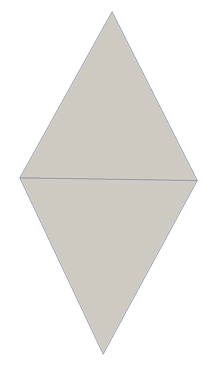
\includegraphics[width=0.19\textwidth]{simulation/tet_cut1}\label{fig:tet_cut1}}
  \hfill%
  \subbottom[]{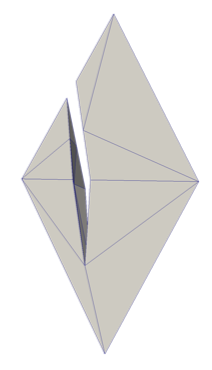
\includegraphics[width=0.19\textwidth]{simulation/tet_cut2}\label{fig:tet_cut2}}
  \hfill%
  \subbottom[]{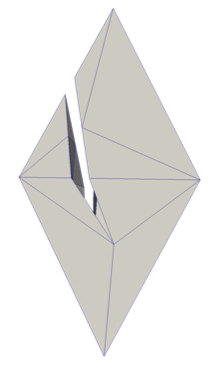
\includegraphics[width=0.19\textwidth]{simulation/tet_cut3}\label{fig:tet_cut3}}
  \hfill%
  \subbottom[]{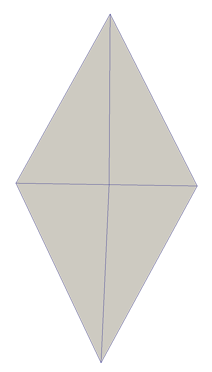
\includegraphics[width=0.19\textwidth]{simulation/tet_cut4}\label{fig:tet_cut4}}
  \hfill%
  \subbottom[]{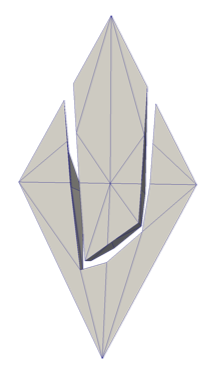
\includegraphics[width=0.19\textwidth]{simulation/tet_cut5}\label{fig:tet_cut5}}
  \caption{This figure shows 2 tetrahedra (\emph{i}), top and bottom, and a cut that intersects an edge separating the 2 tetrahedra (\emph{ii}) curves inside the bottom one (\emph{iii}) and exits intersecting the same edge. When the second cut is detected, the mesh is refined as seen in (\emph{iv}), and the cut reapplied (\emph{v}).}\label{fig:tet_cuts}
\end{figure}

The methods of the cutting modules could result under certain conditions in some flat tetrahedra. The refinement techniques are used to clean the mesh from such anomalies. A case is shown in \autoref{fig:flat_tet}.

\begin{figure}
  \centering%
  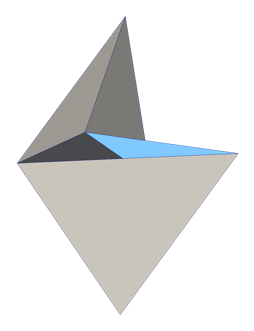
\includegraphics[width=0.3\textwidth]{simulation/tet_flat1}\label{fig:tet_flat1}
  \hspace{10ex}
  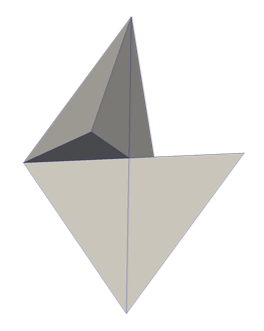
\includegraphics[width=0.3\textwidth]{simulation/tet_flat2}\label{fig:tet_flat2}
  \caption{In this figure, the left mesh (3 tetrahedra) admits a single flat cell shaded in blue, on the right the cluster of affected cells are removed and replaced with an equivalent set (4 tetrahedra) without any flat cells.}\label{fig:flat_tet}
\end{figure}

% In the Figure, the left mesh (3 tetrahedra) admits a single flat cell shaded in blue, on the right the cluster of affected cells are removed and replaced with an equivalent set (4 tetrahedra) without any flat cells.

\subsection{Fast Incremental Solver}
\begin{minipage}{0.6\linewidth}
  The team further developed programmatic representations of different types of cutting models in order to facilitate the interface between the cutting module and the user interface. These representations can capture blades of any curvature with virtually no additional interventions from the User Interface (UI). The representation discretizes a cutting tool and its swept surface as a set of segments and triangles capturing the motion and the physical position of the blade. The figure on the right shows the simplest form of such a representation with a starting and ending blade positions (green and red respectively).
\end{minipage}
\hfill%
\begin{minipage}{0.4\linewidth}
  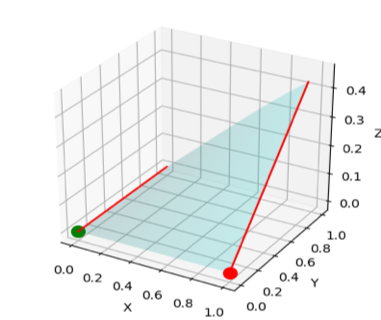
\includegraphics[width=\linewidth]{simulation/incremental}\label{fig:incremental}
\end{minipage}

The key challenge to a fast incremental solver is the fine-grained communication with a Bounding Volume Hierarchy (BVH), a powerful data structure for tracking geometric objects and accelerating geometric operations such as triangle-segment intersections ubiquitous in the cutting module. A programming interface (API) was designed and implemented to open the BVH to the cutting module and allow it to communicate information back to BVH. In particular, the BVH API allows the cutting module to determine which edges and faces of the mesh have been cut by a particular sweep of a cutting tool, as well as the geometries of these intersections, in logarithmic complexity.

Furthermore, cutting the mesh produces modifications and this information must be communicated with the other modules of the system. The BVH module requires information about all changes in the mesh to be able to update and restructure the hierarchy so it is synchronized with the base mesh to continue supporting intersection queries. In addition, the UI requires the new surface triangles that are created as the mesh opens up after the cut in order to render the new shape of the mesh. These changes are also important for updating the factorization of the finite element stiffness system matrix, where a change in the mesh necessarily affects the behavior of the mesh and its response to applied forces.

The efficient collection and communication of these changes (also known as topology deltas) is key to the successful integration of the different aforementioned modules. Such a system was implemented within the cutting module and their communication between the different modules tested and debugged. The system keeps track of all new tetrahedra along with the new and deleted edges and faces per cutting step and communicates the strict necessary to the other modules.

The result is a complete system controllable through a UI that can load and cut open a volumetric mesh in real time. Cuts can have sharp curvatures---sharper than those that are resolved by the geometric mesh; cuts are incremental: they can completely separate the 3D mesh or only partially open it; cuts can also intersect each other. We believe these capabilities surpass the state of the art in this area and our early presentations of the system at international conferences have been very well received, with leading groups from around the world requesting access to the system. Below is a screenshot from the running system. Sample animation videos are available at \url{https://www.dropbox.com/s/ly53lbgmy1m2aw2/animm-4cuts.avi} and \url{https://www.dropbox.com/s/rjmw8avzb0dkwpm/animm-liver.avi}.

\vspace{1ex}
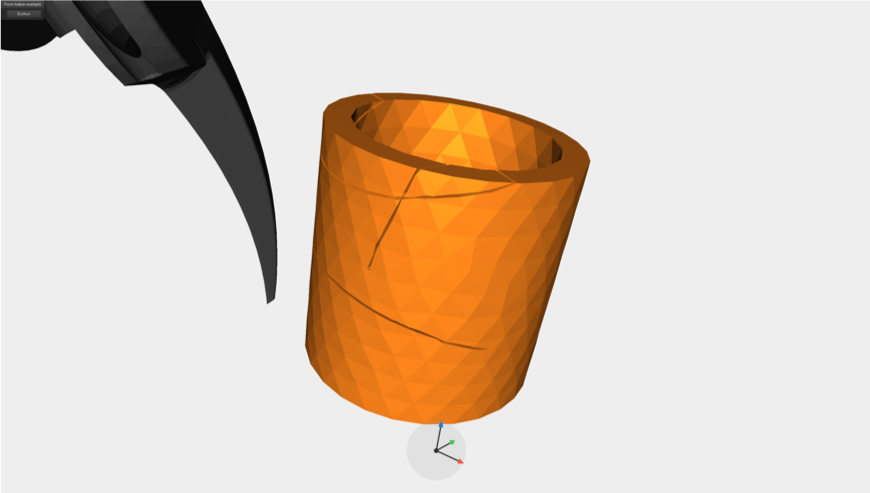
\includegraphics[width=\linewidth,frame]{simulation/endo_cut}

\subsection{Non-linear Solver}
We have started the development of a refinement of our non-linear solver that has the potential to produce two key advantages:
\begin{inparaenum}[(1)]
  \item it allows a straightforward mechanism for trading real-time solution speed and efficiency with solution accuracy.  We have found that when complex maneuvers are performed on a deformable mesh, a reasonably sizeable subset of teteraheda, faces, and edges may be affected. Resolving all these changes to high-accuracy in real time is not possible. Therefore, an elegant solution is to maintain real-time rates of interaction and display, but allow slightly lower fidelity in the rendered deformations.  This lower-fidelity rendering is only transient however. As soon as the complex maneuver that induces large topological changes slows down, the solver “catches up” and is able to resolve the deformation to the desired higher accuracy;
  \item it allows a pre-computed factorization of the system matrix to be reused even when a large portion of the model undergoes large rotations requiring non-linear kinematics to be recomputed for a large set of elements. The system stiffness matrix factorization is updated, very efficiently via low rank updates, only when topological changes are introduced by cutting or suturing.  The refined non-linear solution algorithm is effectively an alternating minimization procedure that alternates on updating nodal positions and element deformations/orientations. The element deformations updates are local in nature, providing a substantial algorithmic benefit. The description of this algorithm and its performance in the context of our overall cutting system will be submitted for publication later this summer.
\end{inparaenum}

\section{GPU Acceleration}
We have continued the development of GPU-accelerated routines for the hierarchical matrix-vector multiplication operations as well as for the low-rank update operations involved in the finite element solution. Our recent publication on this subject was accepted by the prestigious journal ACM Transactions on Mathematical Software, where we have shown that the absolute performance of these operations can very effectively leverage the power of GPUs and, perhaps more importantly, that the optimal linear and log-linear growth of these algorithms allow the scaling of our cutting and suturing models beyond what current state of the art systems can do.  In the next period, we plan to perform an extensive study of system performance with the GPU acceleration enabled on benchmark problems. We plan to submit a publication, along with the demonstration of our system, to document what we believe should be world-record performance.

\hrule%

\section{Discontinuous Finite Elements}
This task is now complete and has been tested on a variety of configurations. The system has the ability to handle a variety of cutting scenarios that introduce different topological configurations of the cut tetrahedra. Different parameters allow the system to handle different physical parameters, involving more or less or more prestress in the material, as well as different geometric configurations. The figure below includes illustrations of discontinuities introduced in volumetric tetrahedral meshes.  When cuts are introduced, edges may be cut twice requiring additional adaptive tetrahedral refinements that are handled by the system transparently.

\begin{figure}
  \centering%
  \setlength{\fboxsep}{0pt}%
  \setlength{\fboxrule}{0.1pt}%
  \fbox{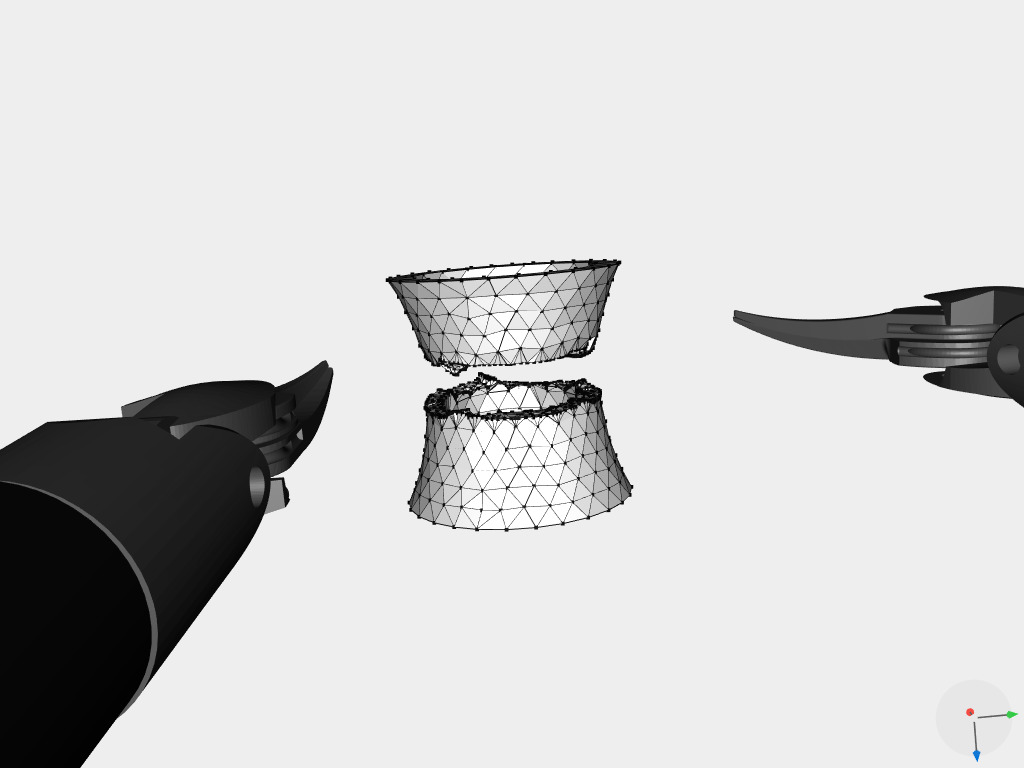
\includegraphics[width=0.32\linewidth]{simulation/snip0}}
  \hfill%
  \fbox{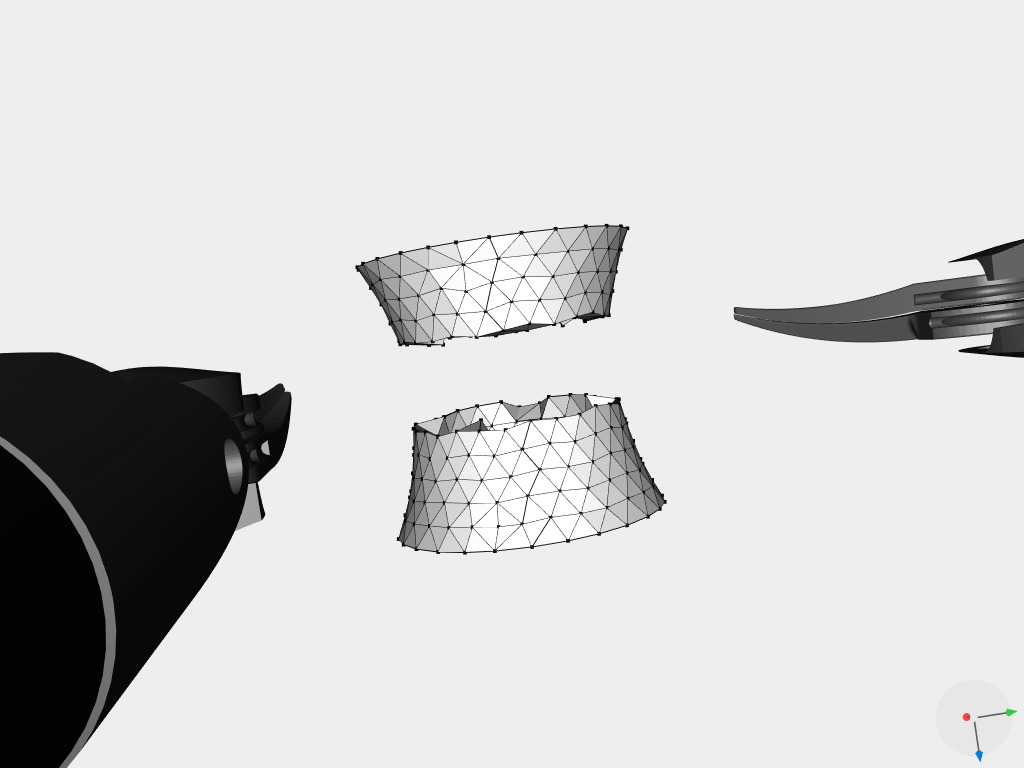
\includegraphics[width=0.32\linewidth]{simulation/snip1}}
  \hfill%
  \fbox{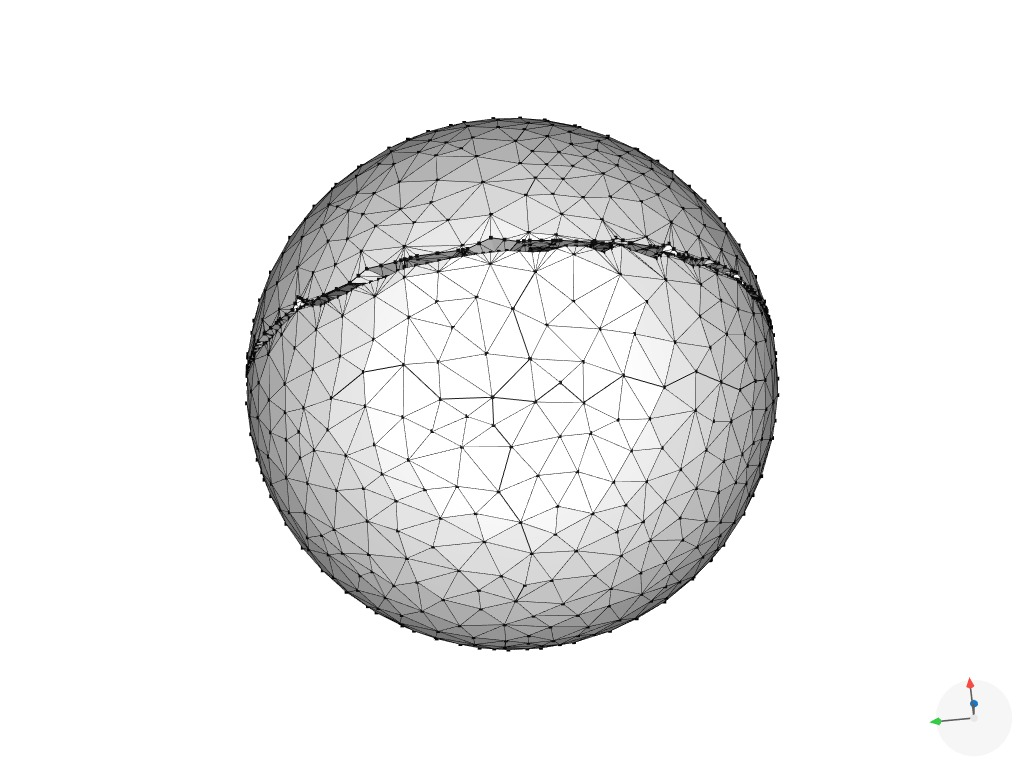
\includegraphics[width=0.32\linewidth]{simulation/snip2}}
  \caption{---}\label{fig:cuts}
\end{figure}

\section{Fast Incremental Solver}
The work on the fast solver has tested the performance of the system on a variety of configurations. The typical cutting scenario involves a deformation of the soft tissue by a tool followed by a snipping motion in the case of scissors, as illustrated below (the transparent triangular surface shows the snipping motion of the blades of the scissors).  Testing with various sequences of snips and cuts was performed.

\begin{figure}
  \centering%
  \setlength{\fboxsep}{0pt}%
  \setlength{\fboxrule}{0.1pt}%
  \fbox{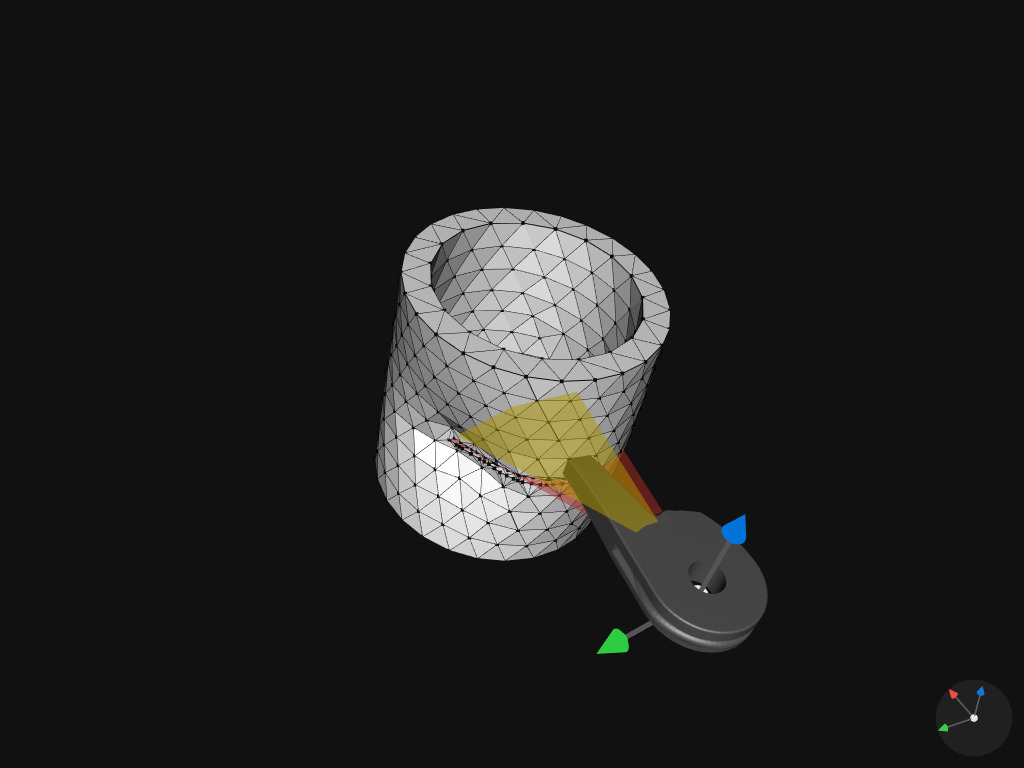
\includegraphics[width=0.5\linewidth]{simulation/snip3}}
  \caption{---}\label{fig:contact}
\end{figure}

The key to fast incremental solution is the efficient two-way fine-grained communication between the finite element cutting system and the collision detection and intersection computation system which incorporates bounding volume hierarchy of the geometric representation. The geometric computation system returns intersection information that is used to build incrementally a set of constraints and/or a set of cuts in the volumetric mesh, and the finite element system returns set of new vertex positions as well as ``topology deltas'' indicating which elements have been removed and how new elements were added instead. This two-way incremental communication was also tested.

Timings of the various steps in the process have been performed. The results of the timings identified one bottleneck that could prevent real-time interaction as the constrains set size increases. Optimizations we performed as a result to remove inactive constraints prior to entering the solution loop. This resulted in a much more responsive system with a stable interaction time for the kinds of meshes needed when cutting urethra and models of similar complexity.

In addition, a hierarchical matrix representation of the system stiffness that replaces the sparse Cholesky factors of the stiffness was also tested and timed. This representation may be used for the solution involving simple deformation constraints and updated, via low-rank matrix updates, to account for cuts introduced. Hierarchical matrix representation is the primary mechanism for getting the solution strategy to run on GPUs, as the sparse matrix factors cannot efficiently take advantage of the many cores of the GPUs.

\section{Non-linear Solver}
We have wrapped up and tested the developments of the non-linear solver algorithm. Our algorithm is particularly designed for real-time interaction as it allows a pre-computed factorization of the system matrix to be reused even when a large portion of the model undergoes large rotations requiring non-linear kinematics to be recomputed for a large set of elements. The alternating minimization procedure used in the solver alternates on updating nodal positions and element deformations/orientations. The element deformations updates are local in nature, providing a substantial algorithmic benefit particularly on GPUs. A GPU kernel to compute the local updates in parallel has been developed to be used in tandem with the stiffness matrix factorization, updated as cuts are introduced.

Fine-tuning and calibrations of the parameters of the non-linear solver were also performed.  The  solver iterates on two types of nonlinearities:
\begin{inparaenum}[(1)]
\item the ``outer'' non-linearity which involves the active set of constrains; the solution algorithm must iterate until this active set is stable; and
\item non-linearity of the deformations for a given set of active constraints; this is the inner loop of the iteration and does not need to be solved to final accuracy until a stable active constraint set has been identified.
\end{inparaenum}

\section{GPU Acceleration}
We have finished the development of algorithms to support the acceleration of the solution computation when running in the presence of GPUs.  The system can now build approximate hierarchical matrix representations of inverses of the stiffness matrices and perform low rank update operations on them in their compressed hierarchical form as the cutting operation progresses. A recent publication documenting various aspects of these developments has been accepted in the flagship SIAM Journal on Scientific Computing. These state-of-the-art algorithms are pushing the boundary of what is possible to do in real time on GPUs, at the fundamental algorithmic level. Their integration in the simulation system is allowing us to scale the simulations to higher resolution and higher fidelity models.

As examples of the high performance of the system, the figure below shows GPU timings and scalability results. The left figure shows the time it takes to construct a hierarchical matrix on a representative problem of various sizes on a P100 Nvidia GPU, while the middle figure shows the corresponding performance achieved on these problems. Problems of size 16,000, which are already useful for high resolution surgical models, achieve a 100\,GFLOPS/s performance. Larger models achieve even higher performance, and the growth in runtime is only log-linear in problem size. The last plot shows a computation of the inverse of a stiffness matrix using an iterative Newton-Schulz method on a problem of size 4,000. Second order convergence is observed, and the whole computation is GPU-resident.

\begin{figure}
  \centering%
  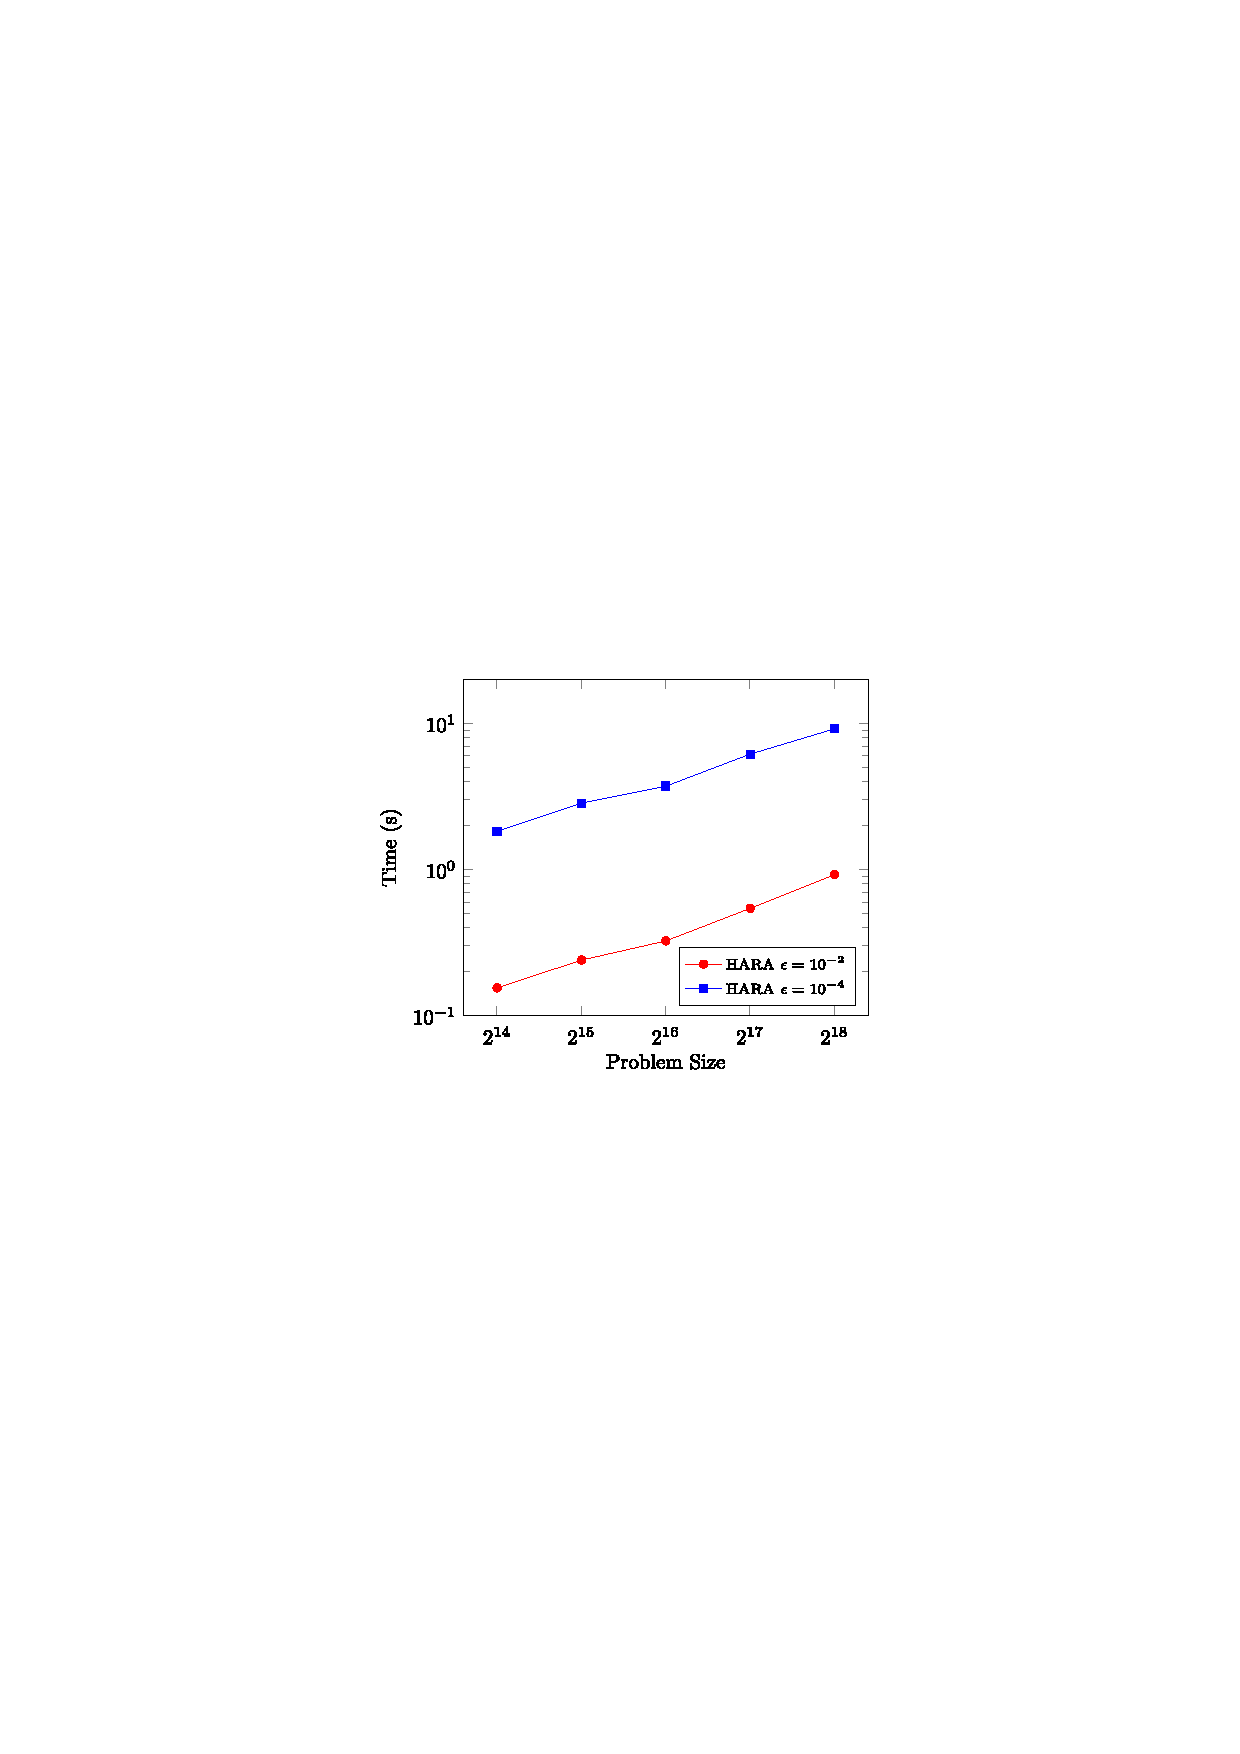
\includegraphics[trim=180 200 160 300,clip,width=0.32\linewidth]{simulation/plot0.pdf}
  \hfill%
  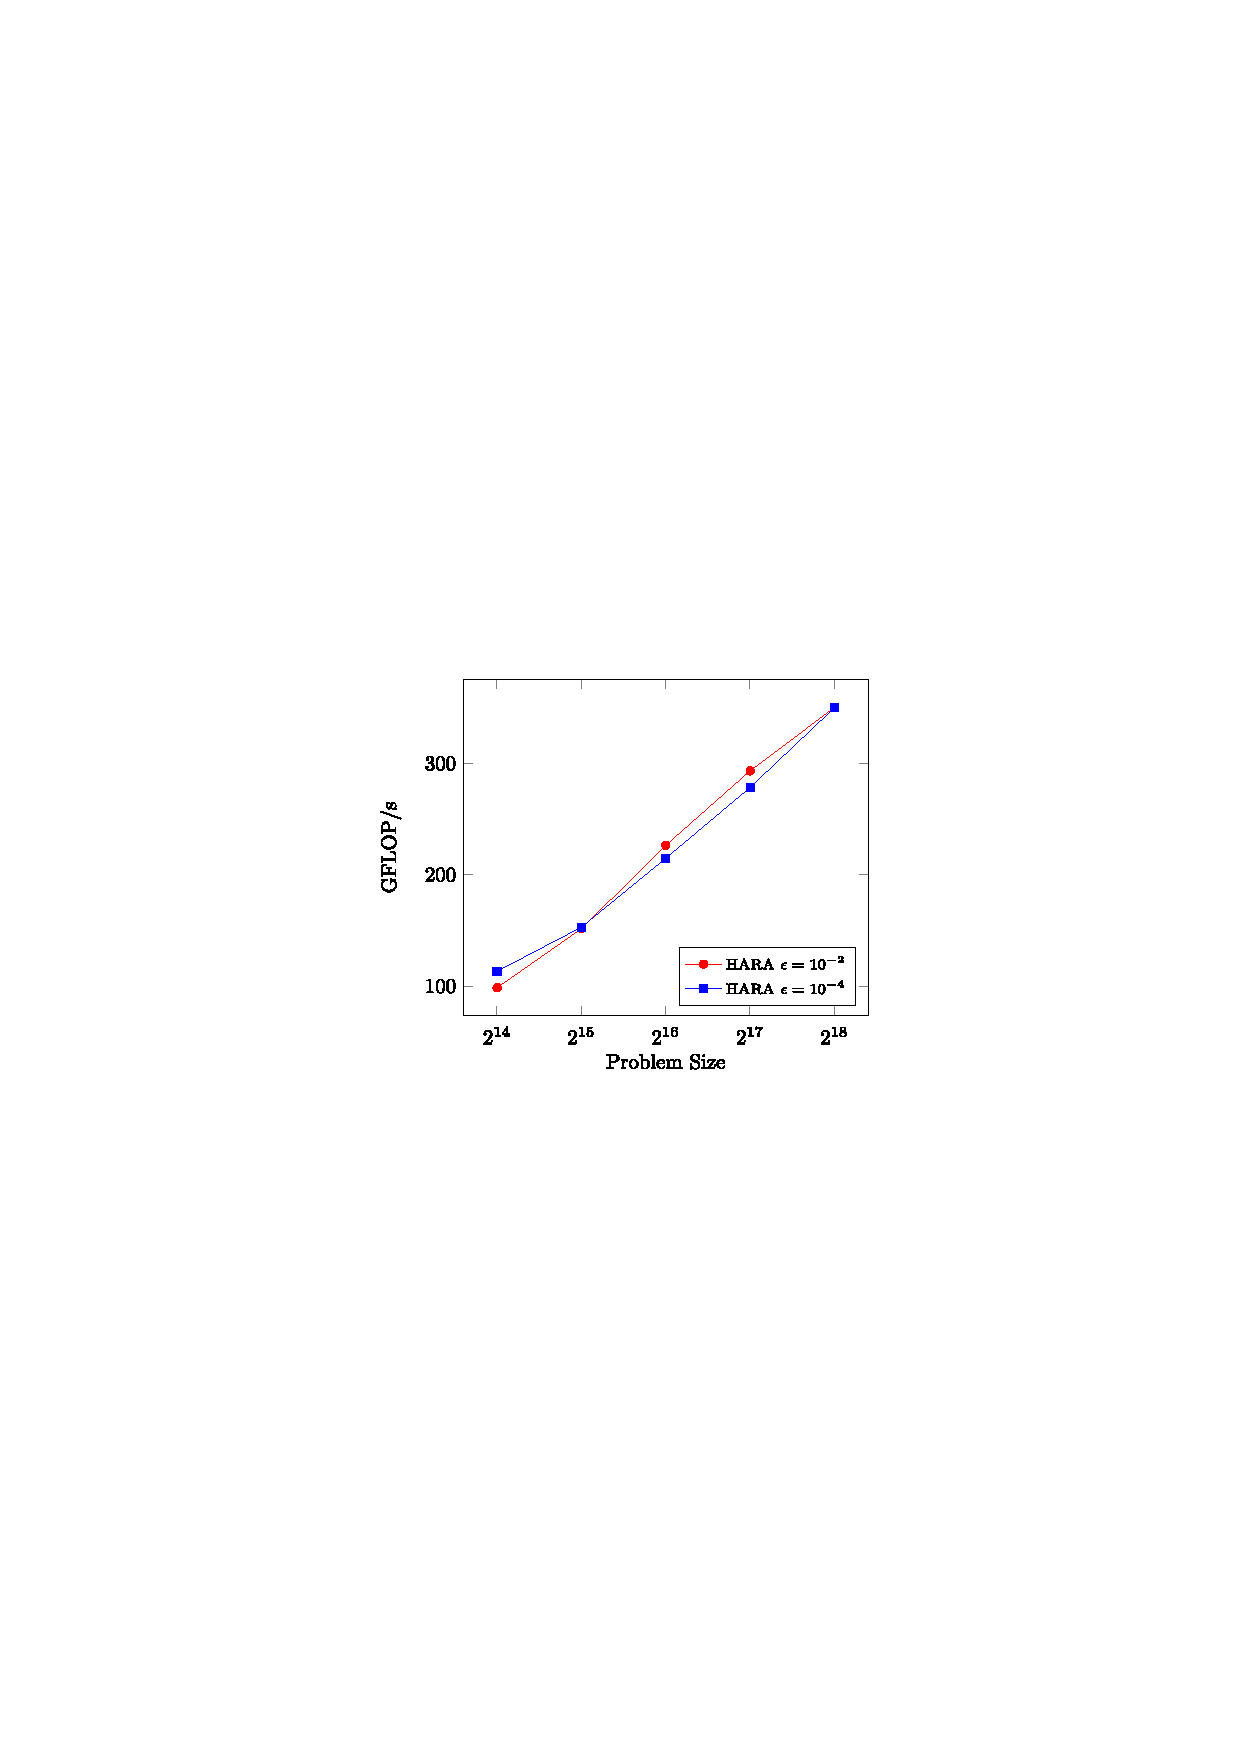
\includegraphics[trim=180 200 160 300,clip,width=0.32\linewidth]{simulation/plot1.pdf}
  \hfill%
  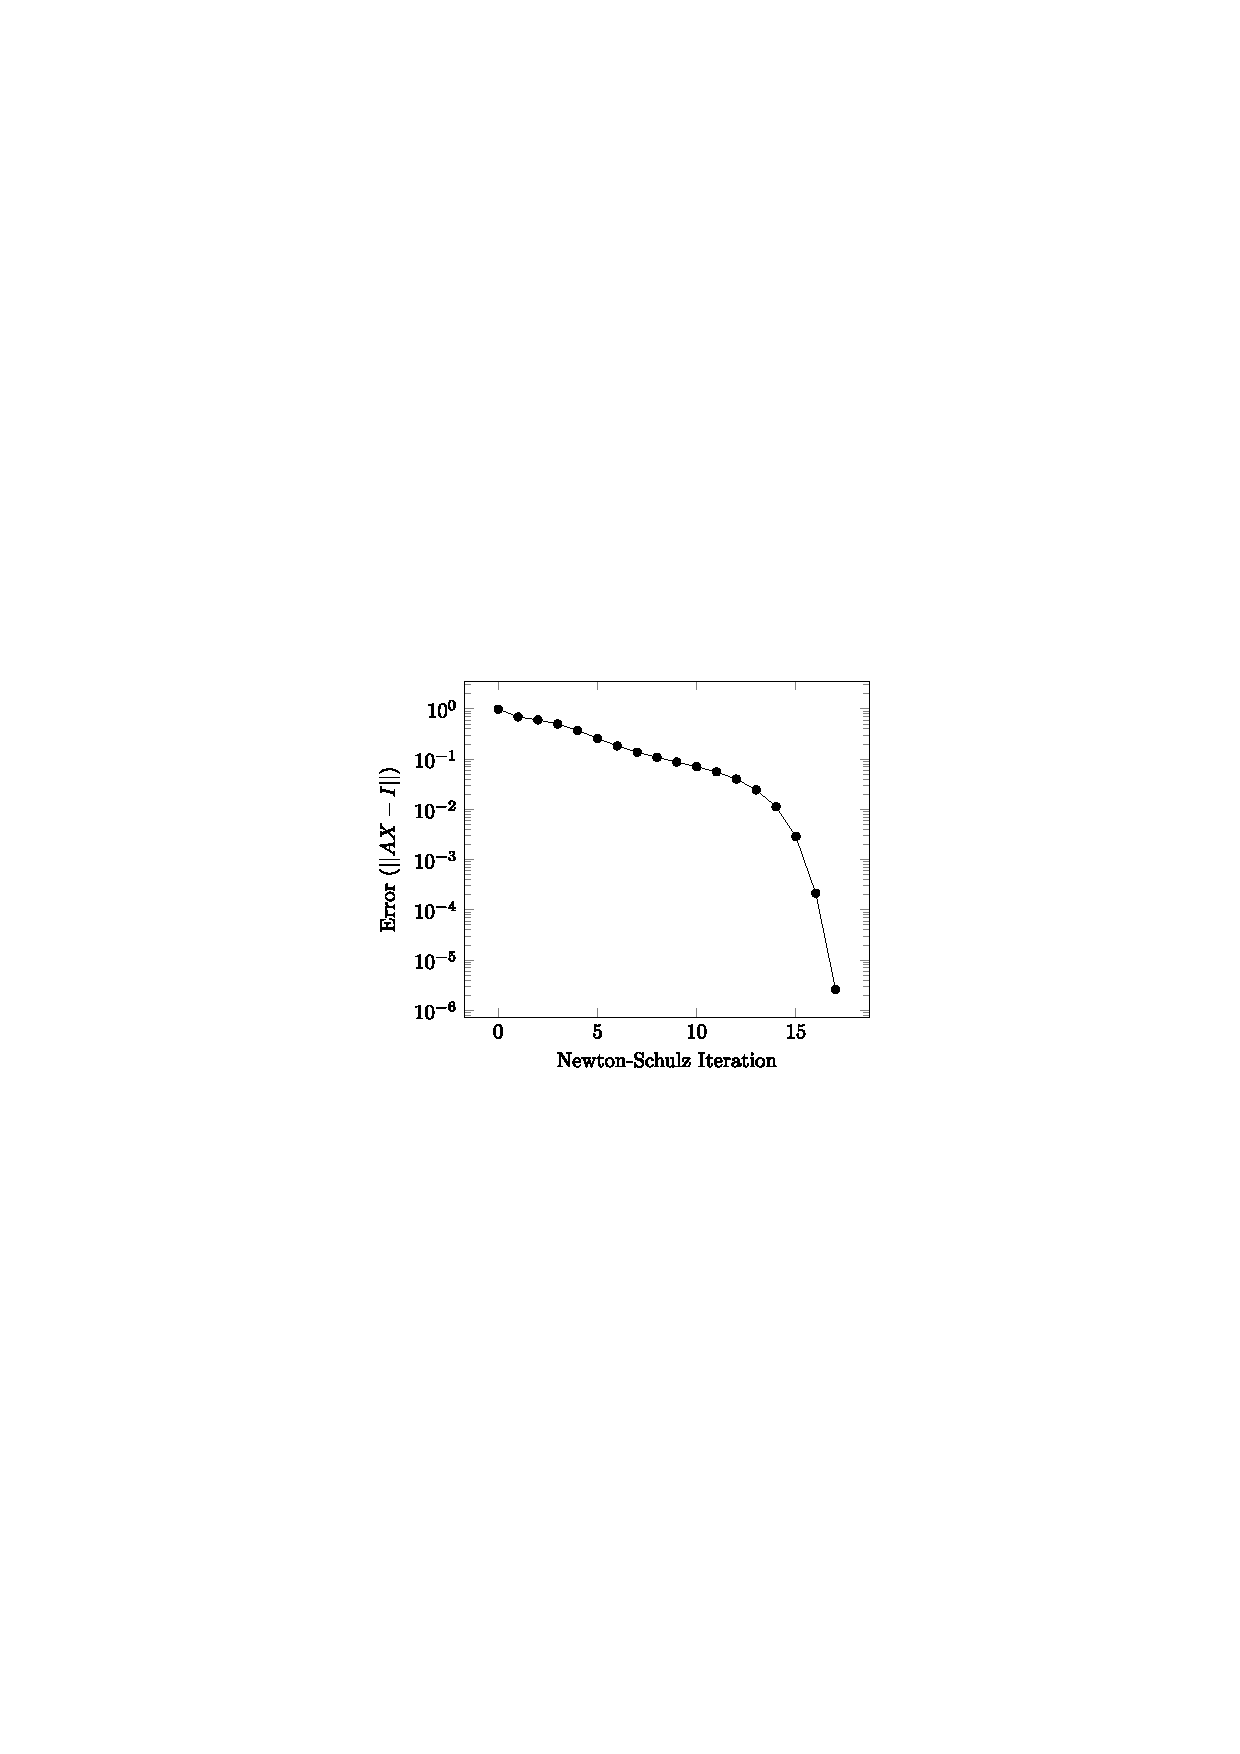
\includegraphics[trim=180 200 160 300,clip,width=0.32\linewidth]{simulation/plot2.pdf}
  \caption{---}\label{fig:plots}
\end{figure}

\clearpage%
